
\newpage
\section{Model package}

In questa sezione descriveremo il package \textbf{Model}.

Questo package contiene le implementazioni dei concetti che riguardano
la pi\`u importante e ricca astrazione del concetto di vertice, del
nostro modello di grafo, delle specializzazioni del concetto di
vertice e di due astrazioni legate alla programmazione funzionale.

\subsection{Supplied Abstractions}

Le astrazioni fornite da questo package sono le seguenti:
\begin{itemize}
\label{itemize:model-supplied-abstraction}
\item fornire l'astrazione di vertice e le sue specializzazioni
  necessarie per implementare gli altri moduli del progetto. Questa
  astrazione pu\`o essere modellata a livello teorico come un
  \emph{abstract data type}, in quanto non siamo interessati che i
  client siano a conoscenza delle specifiche realizzazioni (come
  invece lo sarebbe se fosse stato un \emph{algebraic data type}), ma
  vogliamo usare un approccio trasparente per mantenere flessibile il
  sistema. Le specializzazioni del concetto di vertice che ho
  implementato riguardo il concetto semplice di vertice, di vertice da
  usare in una ricerca \emph{DFS} e nell'algoritmo di Tarjan per la
  ricerca delle componenti fortemente connesse.
\item fornire l'astrazione del grafo, arricchendola con comportamenti
  per poter modificare la struttura del grafo rappresentato e poter
  eseguire delle computazioni su di esso: \`e possibile usare due idee
  prese dal paradigma funzionale per agire sui vertici del grafo ed
  \`e fornita una implementazione dell'algoritmo \emph{DFS}, che espone
  degli \emph{hot spots} in modo da permettere ai client di avere
  gi\`a implementata la struttura dell'algoritmo, fornendo solo il
  comportamento specifico di interesse.
\item nascondere tutti i tipi che implementano i concetti astratti ai
  client di questo package, in modo da utilizzare le astrazioni
  mediante interfaccie e non accoppiando i client con specifiche
  realizzazioni attraverso delle factory 
\item interfacciare le astrazioni di vertice e grafo con gli oggetti
  definiti nel package \emph{DotInterface}, per permettere una
  rappresentazione grafica che cattura le idee definite nell'articolo
  \cite{tellingStories}
\end{itemize}

\subsection{Class diagram}
Il diagramma rappresentato in figura
\ref{fig:vertex-abstraction-interfaces} rappresenta le interfaccie
introdotte in questo package. Procediamo con ordine nel descrivere le
idee principali catturate in ogni contratto:

\begin{figure}
  \centering
  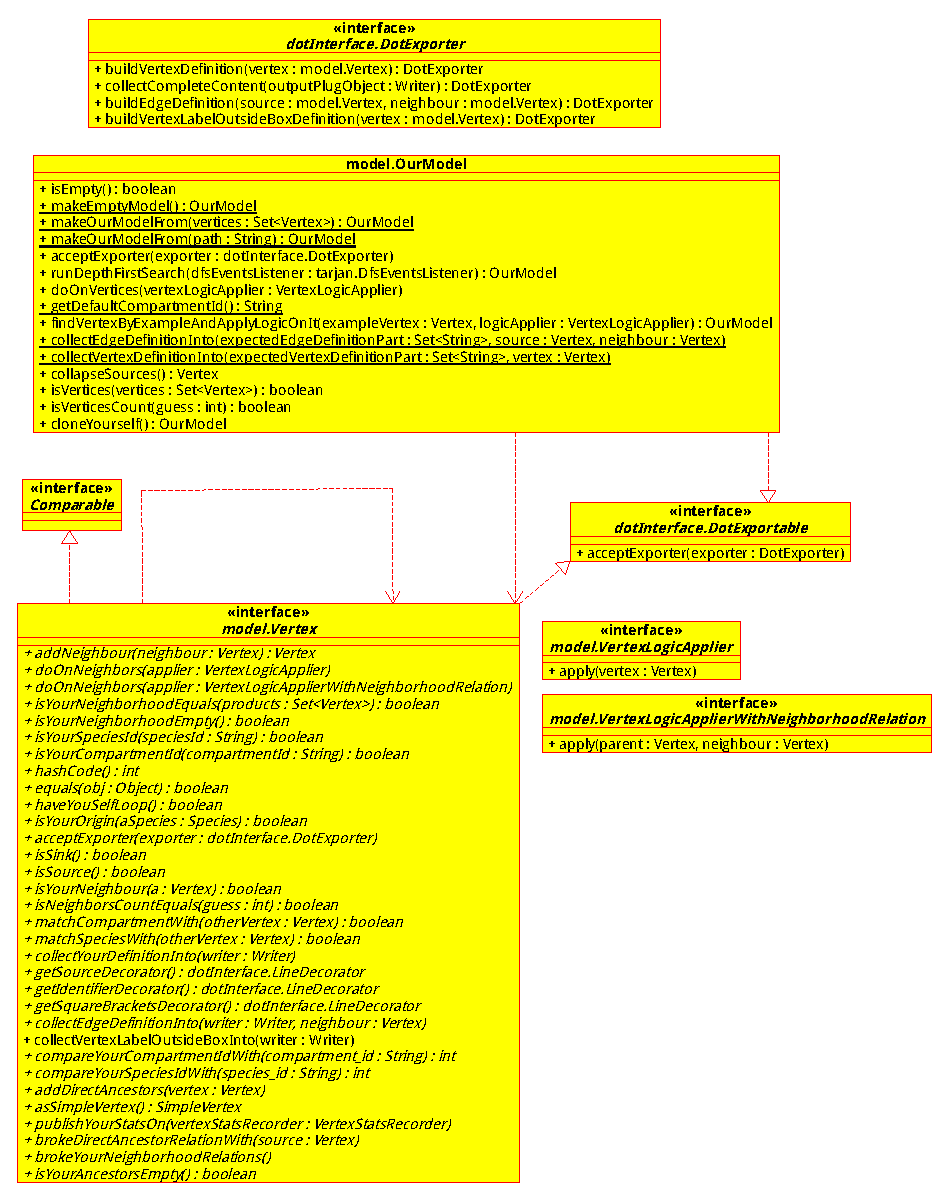
\includegraphics{packages/vertex-interface-class-diagram.eps}
  \caption{Vertex abstraction interfaces}
  \label{fig:vertex-abstraction-interfaces}
\end{figure}

\begin{paragraph}{Vertex}

  L'interfaccia \emph{Vertex} \`e l'astrazione principale dell'intera
  libreria ed \`e molto ricca di contenuto.  Tramite \emph{Vertex}
  possiamo richiedere ad un valido implementatore, di gestire le
  informazioni sul vicinato di un vertice, dando la possibilit\`a sia
  di aggiungere vicini che predecessori (quindi modelliamo sia una
  lista di adiacenza, sia una lista di incidenza). Questo ci permette
  di avere un costo nell'ordine $O(m + n)$ dove $m$ \`e il numero
  totali di archi presenti nel grafo codificato nel nostro modello ed
  $n$ \`e invece il numero di nodi dello stesso. Inoltre, per poter
  collassare le sorgenti in una unica\footnote{aggiungere qui
    riferimento alla descrizione del relativo use case}, \`e possibile
  richiedere la "rottura" della relazione di vicinato per poter
  successivamente cancellare il vertice dal grafo, senza lasciare
  coppie nell'insieme degli archi $E$ che contengono nodi sorgente
  rimossi.

  \emph{Vertex} permette di richiedere informazioni sulle
  caratteristiche del vertice, ad esempio se un vertice \`e sorgente o
  pozzo, qual \`e il suo vicinato, quali sono le informazioni che lo
  distinguono (riferite alla \emph{species} e al \emph{compartment}
  recuperate dal modello SBML di origine). Molti di questi metodi sono
  utilizzati soprattutto nei metodi di unit testing e hanno una firma
  che rispetta i concetti espressi nella sezione
  \nameref{sec:objects-oriented-functional-paradigms}\footnote{in
    questa sezione descrivere perche si e' evitato metodi di get e set
    in benificio di metodi della forma is...()}.

  Tramite questo contratto possiamo interfacciarci con le
  implementazioni definite nel package
  \emph{dotInterface}\footnote{aggiungere qui collegamento con
    nameref}, richiedendo di poter accettare un esportatore per
  costruire un documento in formato \emph{dot}, fornendo gli oggetti
  necessari per la corretta formattazione delle informazioni
  incapsulate nell'oggetto che implementa il contratto
  \emph{Vertex}. Utilizzando solo contratti, siamo in grado di avere
  questi due comportamenti \emph{loosesly coupled}, in quanto
  cambiamenti agli effettivi implementatori dei due contratti, non
  comportano cambiamenti ai metodi definiti nelle interfaccie.

  Una propriet\`a che questo contratto richiede \`e quella di
  riscrivere i metodi \emph{equals} e \emph{hashCode} in modo che
  tutti gli oggetti implementatori di questa interfaccia possano
  essere trattati come \emph{value objects}, non distinguendoli per
  riferimento in memoria (implementazione di default del metodo
  \emph{equals} fornito da \emph{openjdk}), bensi dalle informazioni
  che questi incapsulano (e quindi poter usare \emph{late-binding} ed
  avere comportamento polimorfo in base all'oggetto che riceve i
  suddetti messaggi). Abbiamo effettuato questa scelta in modo da
  poter creare implementatori di \emph{Vertex} all'occorrenza con le
  stesse caratteristiche, senza dover gestire una struttura dati per
  la memorizzazione e la ricerca dell' unico oggetto creato.

  Come ultima propriet\`a, questo contratto impone una relazione
  d'ordine totale sull'insieme degli implementatori, in modo da
  rendere gli algoritmi deterministici nel momento di selezione di
  vertici. Questo \`e stato utile per la stesura dei metodi di unit
  testing.

\end{paragraph}

\begin{paragraph}{OurModel}
  La classe concreta \emph{OurModel} cattura il concetto di grafo da
  utilizzare come modello di dominio per le computazioni descritte nel
  capitolo \ref{chapter:study}.

  La prima responsabilit\`a di \emph{OurModel} \`e quella di fornire
  il comportamento per la costruzione del modello in diverse
  modalit\`a: costruire un modello a partire da un insieme di vertici
  gi\`a costruiti (e, quindi, con le relazioni di vicinato gi\`a
  fissate), oppure a partire da un modello SBML esistente in una path
  del file system.

  Questa classe non solo permette di poter manipolare e rappresentare
  in un "tutt'uno" un grafo, ma espone dei comportamenti fondamentali
  per l'implementazione dei concetti descritti nel capitolo
  \ref{chapter:theoretical-background}.

  Viene fornita la logica per compattare le sorgenti in una unica,
  restituendo una nuova istanza di grafo con la struttura richiesta,
  lasciando immutato il modello di input, dando la possibilit\`a di
  poter continuare ad inviare messaggi al modello originale.

  Un altra importante astrazione che utilizza uno stile funzionale
  permette di poter applicare un comportamento definito dal client di
  \emph{OurModel} su ogni vertice in esso contenuto. Questo \`e stato
  un vero punto di forza che ci ha permesso di aver un codice pulito,
  mantenibile e orientato al testing.

  L'ultimo comportamento che merita attenzione \`e quello di
  templetizzare l'algoritmo di \emph{DFS}, introducendo degli
  \emph{hot spots} sui quali \`e possibile "customizzare" il
  comportamento della ricerca ed implementare delle sue
  varianti. Quelle che abbiamo implementato in questo lavoro sono
  strettamente quelle definite nel capitolo
  \ref{chapter:theoretical-background}, ma questo non limita un
  utilizzatore della libreria di definire il proprio comportamento e
  di usare l'implementazione della ricerca per algoritmi non trattati
  in questo documento.

\end{paragraph}

\begin{paragraph}{Vertex implementors}
  Abbiamo molti comportamenti diversi che vogliamo poter utilizzare
  come istanze dell'astrazione definita dal contratto
  \emph{Vertex}. Il vantaggio di aver implementato il codice
  riferendosi sempre al contratto e non alle singole caratterizzazioni
  ci ha dato l'enorme vantaggio di poter essere trasparenti e poter
  interscambiare questi aspetti specificando solo nel rispettivi
  contesti quale comportamento si preferiva utilizzare, lasciando
  completamente immutato il codice che invece implementa i vari
  algoritmi.

  In questo paragrafo enumeriamo quali sono le caratterizzazioni (il
  \emph{Vector of changes} come viene chiamato da Bruce Eckel in
  \footnote{aggiungere qui il riferimento bibliografico a Thinking in
    Patterns}) e alcune loro propriet\`a.

  La prima caratterizzazione ad esser stata implementata \`e
  \emph{SimpleVertex}, la quale cattura il comportamento di un vertice
  "normale", ovvero l'implementazione pi\`u semplice possibile del
  contratto. Anche se questa pu\`o sembrare scontata, invece \`e il
  building-block utilizzato pi\`u o meno indirettamente anche da
  caratterizzazioni pi\`u complesse. Come vedremo \footnote{nella
    sezione dei patterns inserire un paragrafo sulla comodit\`a di
    utilizzare i wrapper per evitare il problema della fragile base
    class, fare riferimento anche al libro di Josch Block}, queste
  caratterizzazioni avanzate sono dei \emph{wrapper} che delegano
  parte del comportamento alla caratterizzazione \emph{SimpleVertex} e
  ridefiniscono solo il comportamento che differisce da quest'ultima.

  La successiva caratterizzazione introdotta \`e stata
  \emph{DfsWrapperVertex}, la quale permette di associare l'analogo di
  un "timestamp" nel momento in cui la ricerca visita un vertice e nel
  momento in cui la visita abbandona il vertice. Questo ci ha permesso
  di produrre una rappresentazione simile a quella che
  \emph{Papadimitriou} propone nel suo volume \footnote{aggiungere qui
    il riferimento bibliografico al volume di Algorithms e alle pagine
    in cui si evidenzia la coppia di interi} ed analizzata nel
  capitolo \ref{chapter:study}.
\end{paragraph}

